\documentclass[12pt, onside]{article}
\usepackage[utf8]{inputenc}             % UTF8 encoding
\usepackage{parskip}% Extra interlining
\usepackage[margin=0.8in]{geometry}    % Margins
\usepackage[spanish]{babel}


% Header and Footer
\usepackage{fancyhdr}
\setlength\headheight{30pt}
\pagestyle{fancy}
\renewcommand{\headrulewidth}{0.4pt}
\fancyhead{}
\fancyhead[L]{
    \textbf{Prácticas Servicios Telemáticos}
}
\fancyhead[R]{
    Emilio Domínguez Sánchez
}
\fancyfoot{}
\fancyfoot[C]{\thepage}


\usepackage{hyperref}
\usepackage{cleveref}
\usepackage{xcolor}
\usepackage{graphicx}
% Code Listings Configuration File

\usepackage{listings}
\renewcommand{\lstlistingname}{Código}
\crefname{lstlisting}{código}{códigos}
\Crefname{lstlisting}{Código}{Códigos}


\definecolor{background}{rgb}{0.99,0.99,0.99}
\definecolor{mygreen}{rgb}{0.1,0.6,0.1}
\definecolor{mygray}{rgb}{0.5,0.5,0.5}
\definecolor{mymauve}{rgb}{0.58,0,0.82}

\definecolor{codeback}{rgb}{0.85,0,0.85}
\newcommand{\code}{\lstinline[basicstyle=\selectfont, language=C]}

\renewcommand{\lstlistlistingname}{Índice de códigos}
\lstset{ 
  title=Fichero \lstname,          % show the filename of files included with \lstinputlisting; also try caption instead of title
  caption=Fichero \texttt{\lstname},
  captionpos=t,                    % sets the caption-position (b/t)
  frame=TBLR,      	               % adds a frame around the code
  rulecolor=\color{black},         % if not set, the frame-color may be changed on line-breaks within not-black text (e.g. comments (green here))
  numbers=left,                    % where to put the line-numbers; possible values are (none, left, right)
  numbersep=10pt,                  % how far the line-numbers are from the code
  % stepnumber=1,                    % the step between two line-numbers. If it's 1, each line will be numbered
  backgroundcolor=\color{background},
  numberstyle=\small\color{mygray},% the style that is used for the line-numbers
  basicstyle=\scriptsize\selectfont, % the size/type of the fonts that are used for the code
  keywordstyle=\color{blue},       % keyword style
  commentstyle=\color{mygreen},    % comment style
  stringstyle=\color{mymauve},     % string literal style
  breakatwhitespace=false,         % sets if automatic breaks should only happen at whitespace
  breaklines=true,                 % sets automatic line breaking
  keepspaces=true,                 % keeps spaces in text, useful for keeping indentation of code (possibly needs columns=flexible)
  showstringspaces=false,          % underline spaces within strings only
  showspaces=false,                % show spaces everywhere adding particular underscores; it overrides 'showstringspaces'
  showtabs=false,                  % show tabs within strings adding particular underscores
  tabsize=2,	                   % sets default tabsize to 2 spaces
  language=C++,                    % the language of the code
  morekeywords={},            % if you want to add more keywords to the set
  deletekeywords={},            % if you want to delete keywords from the given language
  % escapeinside={----}{----},          % if you want to add LaTeX within your code
  extendedchars=true,              % lets you use non-ASCII characters; for 8-bits encodings only, does not work with UTF-8
  literate=
  {á}{{\'a}}1 {é}{{\'e}}1 {í}{{\'i}}1 {ó}{{\'o}}1 {ú}{{\'u}}1
  {Á}{{\'A}}1 {É}{{\'E}}1 {Í}{{\'I}}1 {Ó}{{\'O}}1 {Ú}{{\'U}}1
  {à}{{\`a}}1 {è}{{\`e}}1 {ì}{{\`i}}1 {ò}{{\`o}}1 {ù}{{\`u}}1
  {À}{{\`A}}1 {È}{{\'E}}1 {Ì}{{\`I}}1 {Ò}{{\`O}}1 {Ù}{{\`U}}1
  {ä}{{\"a}}1 {ë}{{\"e}}1 {ï}{{\"i}}1 {ö}{{\"o}}1 {ü}{{\"u}}1
  {Ä}{{\"A}}1 {Ë}{{\"E}}1 {Ï}{{\"I}}1 {Ö}{{\"O}}1 {Ü}{{\"U}}1
  {â}{{\^a}}1 {ê}{{\^e}}1 {î}{{\^i}}1 {ô}{{\^o}}1 {û}{{\^u}}1
  {Â}{{\^A}}1 {Ê}{{\^E}}1 {Î}{{\^I}}1 {Ô}{{\^O}}1 {Û}{{\^U}}1
  {œ}{{\oe}}1 {Œ}{{\OE}}1 {æ}{{\ae}}1 {Æ}{{\AE}}1 {ß}{{\ss}}1
  {ű}{{\H{u}}}1 {Ű}{{\H{U}}}1 {ő}{{\H{o}}}1 {Ő}{{\H{O}}}1
  {ç}{{\c c}}1 {Ç}{{\c C}}1 {ø}{{\o}}1 {å}{{\r a}}1 {Å}{{\r A}}1
  {€}{{\euro}}1 {£}{{\pounds}}1 {«}{{\guillemotleft}}1
  {»}{{\guillemotright}}1 {ñ}{{\~n}}1 {Ñ}{{\~N}}1 {¿}{{?`}}1
}

\usepackage[binary-units=true]{siunitx}
\usepackage{multirow}



\newcommand{\key}{\textsc}
\newcommand{\file}{}
\newcommand{\DNS}{DNS}
\newcommand{\HTML}{HTML}
\newcommand{\HTTP}{HTTP}
\newcommand{\HTTPs}{HTTPs}
\newcommand{\GET}{GET}
\newcommand{\POST}{POST}
\newcommand{\Clang}{C}
\newcommand{\Cplusplus}{C++}
\newcommand{\TCP}[0]{TCP}
\newcommand{\SMTP}{SMTP}
\newcommand{\POP}{POP}
\newcommand{\IP}{IP}
\newcommand{\IPsec}{IPsec}



\begin{document}
\begin{titlepage}
    \begin{center}
        \vspace*{1cm}
        
        \Huge \textbf{Servicios Telemáticos}
        
        \vspace{0.5cm}
        \LARGE Práctica Final
        
        \vspace{0.5cm}
        
        \Large Entrega Anticipada
        
        \vspace{0.5cm}
   		
        \vfill
        
        %Obor XY
        \vspace{0.8cm}
        \Large
            \begin{flushright}
              	\begin{tabular}{lr}
                  Autor:        & Emilio Domínguez Sánchez\\
                  Convocatoria: & Junio 2020\\
                  Grupo:        & 1.4 \\
                \end{tabular}
            \end{flushright}
        \vspace{0.5cm}
        
    \end{center}
\end{titlepage}

\newpage
\tableofcontents
\newpage

\section{Introducción}
La asignatura de Servicios Telemáticos del grado en Ingeniería Informática consta de una parte práctica que consiste en configurar y poner en marcha un conjunto de servicios telemáticos. El enunciado de la práctica
describe los objetivos. En esta memoria se recoge la implementación del enunciado así como el proceso de toma de decisiones.


%\section{Escenario Desarrollado y Versiones del Software}
%\section{Configuraciones}

\section{Servidor Web \HTTP}
\subsection{Introducción}
Implementar y desplegar un servidor {\HTTP} es la tarea principal de estas prácticas. De aquí en adelante, cuando hablemos del servidor nos referiremos a la implementación en lenguaje {\Clang} que hemos llevado a cabo.


\subsection{Usos de \Cplusplus}
Como comentaba, este apartado de prácticas debía realizarse en \Clang. Sin embargo, comenté con mi profesor de prácticas la posibilidad de utilizar \Cplusplus utilizando las mismas llamadas al sistema. Sin embargo, para cumplir con los requisitos de la entrega he mantenido el código como si fuese \Clang. En ese sentido, el grueso del programa es código \Clang. En concreto, he utilizado \Cplusplus para

\begin{itemize}
\item Una clase para imprimir los registros. Permite escribir al registro utilizando la sintaxis que muestro en el \cref{lst-log}.

\item Y en algunas funciones para pasar algunos valores por referencia. Cuando se quiere pasar por referencia un puntero en \Clang, la sintaxis no es cómoda.
\end{itemize}

\begin{lstlisting}[caption=Uso de las clases \code{log} y \code{logerr}, label=lst-log]
Code:   log << "alberto, tenemos un problema de tipo " << type << endl;
Output: INFO(socket ---): alberto, tenemos un problema de tipo ---
Code:   log << endl;
Output:
Code:   log << "mensaje de log 1" << endl;
        log << "mensaje de log 2\n";
Output: INFO(socket ---): mensaje de log 1
        INFO(socket ---): mensaje de log 2
Code:   logerr << "falló una llamada al sistema" << endl;
Output: ERROR: errno=--- exiting pid=---: falló una llamada al sistema
Code:   logerr << "problemas Mike!" << endl << panic();
Output: ERROR: errno=--- exiting pid=---: problemas Mike!
-> Program finishes execution with code -1
\end{lstlisting}


\subsection{Inicio del servidor}
El objetivo básico de un servidor web http es recibir peticiones, que vendrán en forma de un mensaje \key{HTTP request}, y tratarlas. Normalmente, tratarlas significa devolver un recurso al que se intenta acceder.

La función \code{main} del servidor se encuentra dentro del fichero \file{main.cpp}. Al inicio del programa (\cref{lst-daemon}), el objetivo es que el servidor sea ejecutado desde la terminal y funcione como un demonio (es decir, en segundo plano). Para ello, creamos un hijo e ignoramos la señal \key{SIGHUP}% a footnote follows
\footnote{La señal \key{SIGHUP} es una señal que se envía a un proceso cuando la terminal que lo controla finaliza.}.
El proceso padre finaliza automáticamente para devolver el control a la terminal.

\lstinputlisting[linerange={48-59}, label=lst-daemon]{src/main.cpp}

Cuando el servidor recibe una nueva conexión {\TCP} de un cliente, crea un proceso hijo que se encarga de atenderlo y espera hasta recibir otra conexión (\cref{lst-parent-behaviour}).

\lstinputlisting[linerange={61-91}, label=lst-parent-behaviour]{src/main.cpp}

\subsection{Intercambio de mensajes}
La complejidad del servidor está en el trabajo que realiza el proceso para atender al cliente. La función {\Clang} que maneja la conversación es \code{deal_with_client}.

% Apreciaciones Técnicas:
\begin{itemize}
\item Para la lectura se utiliza un buffer de \SI{8}{\kibi\byte}. El servidor lee (\cref{lst-header-reading}) datos de la conexión {\TCP} hasta completar la cabecera de un mensaje {\HTTP} (indicada por la secuencia \code{"\r\n\r\n"}).

\item Tras completar la cabecera de un mensaje, se interpreta la primera línea, llamada \key{status-line} en el protocolo {\HTTP}, para determinar el tipo de mensaje y llamar a una función que lo procese (\cref{lst-request-line}). Esto implica que la cabecera ha de caber en el buffer. Es decir, hay un límite de \SI{8}{\kibi\byte} para el tamaño de la cabecera; y el servidor enviará un mensaje de error en caso de que se supere este tamaño. En la práctica es más que suficiente. Ningún mensaje, aún usando todos los campos disponibles en el protocolo {\HTTP}, utilizaría tanto espacio.

\item El servidor acepta mensajes de tipo {\GET} y {\POST}. Del campo de cabecera \key{content-length} obtiene el tamaño del cuerpo del mensaje, que incorpora al buffer.

\item El servidor no conoce el tamaño de la cabecera de antemano, lo que significa que es posible leer más bytes que los que ocupa un mensaje% a footnote follows
\footnote{Enviar dos mensajes antes de recibir la respuesta del primero se llama \key{pipelining}. Según nuestras pruebas, la versión de \code{firefox} que utilizamos en la máquina virtual no implementa \key{pipelining}.}.
Las funciones \code{process_get} y \code{process_post} devuelven un referencia al primer byte que no formaba parte de su mensaje. La función \code{deal_with_client} lo utiliza para completar la cabecera del siguiente mensaje. De esta manera, la función \code{deal_with_client} no necesita inspeccionar la cabecera (\cref{lst-buffer-adaptation}).
\end{itemize}

\lstinputlisting[linerange={368-408}, label=lst-header-reading]{src/message_processing.cpp}
\lstinputlisting[linerange={418-431}, label=lst-request-line]{src/message_processing.cpp}
\lstinputlisting[linerange={433-450}, label=lst-buffer-adaptation]{src/message_processing.cpp}


\subsection{Persistencia}
Como comentábamos en la sección anterior, el servidor está preparado para aceptar más de un mensaje en la misma conexión. Es lo que se conoce como persistencia en el protocolo {\HTTP}. Las funciones que inspeccionan la cabecera comprueban si el cliente busca mantener la conexión según el valor de la línea de cabecera \key{Connection} y la versión {\HTTP} (el protocolo \key{{\HTTP}/1.0} no se diseñó enfocado a persistencia).

El servidor se ha configurado con un timeout de \SI{5}{\second} que anuncia en la cabecera \key{Keep-Alive}. Se trata del máximo tiempo que el servidor mantendrá la conexión abierta antes de recibir el primer byte del siguiente mensaje (como especifica el protocolo). No obstante, incurrimos en un riesgo de bloqueo si no incluimos otro timeout cuando se espera para completar un mensaje. Un cliente malintencionado podría dejar una conexión abierta indefinidamente, lo que se traduce en un riesgo de negación de servicio (\key{DoS}). Por tanto, hemos incluido un timeout de \SI{1}{\second}.

\subsubsection{Tiempos de timeout en la lectura de cabecera}
Para el control de los tiempos de timeout hemos utilizado la llamada al sistema \code{select} de linux. Es una directiva de sincronización que permite bloquearse a la espera de datos de un \key{socket} durante un tiempo determinado.

La implementación del timeout entre mensajes se puede ver en el \cref{pre-header-timeout}. Es importante ver que hay una comprobación antes sobre el tamaño del buffer de lectura. El motivo es el que ya hemos comentado. Puede ser que hayamos leído parte del mensaje siguiente (incluso entero), en cuyo caso no tenemos por qué esperar.

La implementación del timeout para completar la cabecera se puede ver el \cref{header-timeout}. En ambos casos, si el cliente no envía datos en el tiempo establecido se aborta la conexión. En el caso de que no haya comenzado un mensaje, se trata de un corte normal. En cambio, si ya había comenzado el mensaje y no nos ha llegado el resto del mensaje puede ser que la conexión funcione mal o que sea el cliente el que funcione incorrectamente. En cualquier caso, cortamos la conexión y terminamos con un código de error.

\lstinputlisting[linerange={356-367}, label=pre-header-timeout]{src/message_processing.cpp}
\lstinputlisting[linerange={382-382, 399-407}, label=header-timeout]{src/message_processing.cpp}

\subsubsection{Tiempos de timeout en la lectura del cuerpo del mensaje}
Para aquellos mensajes que contienen un cuerpo (mensajes {\POST} principalmente) también tenemos que controlar el timeout si intentamos leer más datos. Si no, corremos el riesgo de mantener un hilo infinitamente abierto ante un error o un cliente malintencionado. Se hace de forma similar al \cref{header-timeout} pero dentro de las funciones \code{process_get} y \code{process_post}.

\subsubsection{Manejo de las cabeceras \key{Connection} y \key{Keep-Alive}}
El protocolo {\HTTP} exige al servidor que informe al cliente si va a mantener la conexión abierta y cuánto tiempo asegura que lo hará% a footnote
\footnote{Aunque el servidor intente mantener siempre la conexión abierta, puede no poder hacerlo por dos motivos. Porque el cliente pida mantenerla cerrada o porque haya que abortar la conexión, por ejemplo tras un error de formato.}
. Lo primero se hace a través de la cabecera \key{Connection}, que puede tomar los valores \key{close} o \key{keep-alive}. El tiempo se especifica en la cabecera \key{keep-alive}. En nuestra implementación, las funciones que envían ficheros reciben un parámetro que indica si la conexión se mantendrá abierta.

\subsection{Métodos {\GET} y {\POST}}
La funciones \code{process_get} y \code{process_post} inspeccionan del buffer de lectura un mensaje (tipo {\GET} o {\POST}), leen datos del socket hasta completar el cuerpo del mensaje y devuelven el recurso que pide el cliente en forma de un mensaje \key{{\HTTP} response}. En caso de que el mensaje no cumpla el formato o se produzca un error, se devuelve el mensaje de error que indique el protocolo y dependiendo del caso se aborta la ejecución.

Hemos aplicado el siguiente criterio para el corte de la conexión. Si el error es de formato, se considera que no se puede determinar dónde acabaría el mensaje y empezaría el siguiente, y por tanto se aborta la conexión. Lo mismo sucede si se produce un error interno; por ejemplo, por un fallo de una llamada al sistema. En cambio, un error como intentar acceder a un recurso que no existe se considera un error leve. Se devolvería un mensaje con el famoso código {\HTTP}, \key{404 Not Found}, y se procesaría el siguiente mensaje. Se puede ver la implementación de la función \code{process_get} en el \cref{lst-process-get}.

\lstinputlisting[linerange={183-253}, label=lst-process-get]{src/message_processing.cpp}

La función \code{process_post} se comporta de manera similar a la hora de inspeccionar la cabecera, pero la funcionalidad es limitada. Al tratarse de un proyecto de prácticas, el contenido de prueba del servidor solo contiene un formulario {\HTML}. Si se recibe la cadena \code{"email=emilio.dominguezs%40um.es"} devuelve una página de felicitación (\cref{lst-post-check}).

\lstinputlisting[linerange={331-337}, label=lst-post-check]{src/message_processing.cpp}


\subsection{Mensajes {\HTTP} Response}
La función \code{send_static_file} envía un fichero del sistema a través de un mensaje {\HTTP}. Es una función genérica a la que llaman \code{process_get}, \code{process_post} y otras funciones que envían mensajes de error (como \code{send_bad_request}).

La función utiliza un buffer de escritura de $2\cdot \SI{8}{\kibi\byte}$ para poder hacer lecturas (de disco) y escrituras de \SI{8}{\kibi\byte} y minimizar las llamadas al sistema.

\begin{itemize}
\item Mientras el buffer no contenga más de \SI{8}{\kibi\byte} y no se haya leído el fichero al completo, se hace una operación de lectura de \SI{8}{\kibi\byte} del fichero (la operación puede leer menos datos). Como el buffer es de $2\cdot\SI{8}{\kibi\byte}$, siempre hay espcacio para los datos.

\item Mientras el buffer contenga más de \SI{8}{\kibi\byte} o el fichero se haya leído completamente y queden datos por enviar, se ejecuta una operación de escritura de \SI{8}{\kibi\byte}. A continuación se desplaza el exceso de datos al comienzo del buffer para mantener todo el espacio libre a continuación del espacio usado.
\end{itemize}

\lstinputlisting[linerange={15-30,101-181}, label=lst-send-static]{src/message_processing.cpp}

\subsection{Otras anotaciones sobre el código fuente}
Esta sección está dedicada a partes del código que no forman parte de la lógica principal del programa.

\begin{itemize}
\item El fichero \file{http\_parsing.cpp} contiene funciones que sirven para separar los campos de un mensaje {\HTTP}. El mensaje original se modifica y se insertan caracteres nulos en el lugar de algunos delimitadores y se devuelven referencias al caracter donde empezaba cada campo. Como se mantienen referencias al mensaje original, el código es muy eficiente, pero al leer información en el buffer encima de la información actual las referencias se vuelven inválidas. Las funciones también comprueban fallos en el formato de la cabecera.

\item El fichero \file{defs.hpp} contiene definiciones generales para el servidor. Por ejemplo, permite a un usuario cambiar los tiempos de timeout o las asociaciones \key{MIME} que identifican el tipo de fichero según su extensión.
\end{itemize}

\subsection{Mejoras}
Esta sección está pendiente. En la entrega de final incluirá las mejoras que se hayan implementado.
%TODO


\subsection{Ejemplos de funcionamiento y capturas del tráfico de red}
En el archivo \file{tests/capture-global.pcapng} se muestra una captura del funcionamiento del servidor tomada con Wireshark. En las fotos que presentamos hemos aplicado el filtro
\begin{center}
    \lstinline[language=java, basicstyle=\normalsize]
    {http || tcp.flags.syn==1 || tcp.flags.fin==1 || tcp.flags.reset==1}
\end{center}
para mostrar solo los mensajes {\HTTP} y la apertura y el cierre de la conexión. A continuación detallamos el contenido.

\begin{itemize}
\item [\cref{img-cap-normal}] Una prueba de los mensajes intercambiados para cargar la página de inicio e introducir un correo electrónico. Puede servir para verificar la persistencia, viendo como el servidor mantiene la conexión abierta unos segundos esperando a la segunada acción.

\begin{figure}[h]
    \centering
    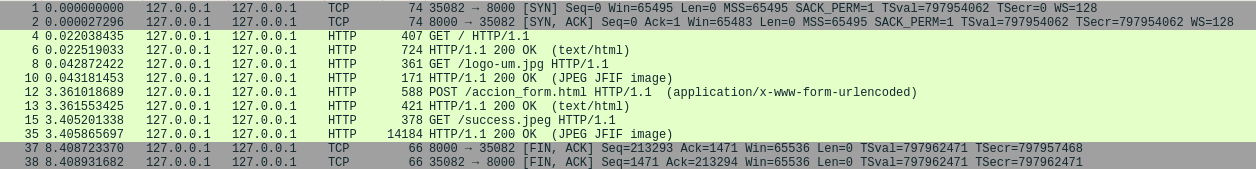
\includegraphics[width=0.95\textwidth]{tests/capture_normal.png}
    \caption{Intercambio de mensajes sin errores.}
    \label{img-cap-normal}
\end{figure}

\item [\cref{img-cap-malfunctioning}] Una prueba de algunos mensajes de error. Muestra un \key{404 Not Found} y un \key{415 Unsupported Media Type}. Además, también muestra la robustez del servidor. Ante un {\POST} de más de \SI{8}{\kibi\byte}, que hemos simulado introduciendo $9000$ caracteres en el campo del correo, devuelve un mensaje \key{413 Request Entity Too Large} y corta la conexión% a footnote
\footnote{Aunque como hemos explicado antes el servidor está preparado para procesar mensajes de tamaño arbitrario leyéndolos en bloques de \SI{8}{\kibi\byte}, hemos establecido el máximo en \SI{8}{\kibi\byte}.}
.

\begin{figure}[h]
    \centering
    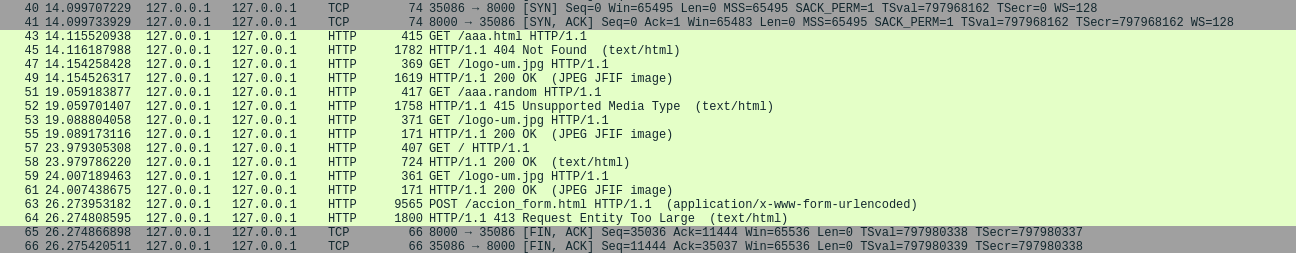
\includegraphics[width=0.95\textwidth]{tests/capture-malfunctioning.png}
    \caption{Intercambio de mensajes de error.}
    \label{img-cap-malfunctioning}
\end{figure}

\item [\cref{img-cap-pipelining}] Una captura probando que el servidor acepta \key{pipelining}. Como el navegador no hacía \key{pipelining}, lo hemos probado utilizando el script del \cref{lst-pipelining-shell}. En un solo paquete {\TCP} se reciben $4$ mensajes {\GET} que el servidor responde en orden. Mediante los mensajes de log se vio que los $4$ mensajes se leyeron en la misma operación de lectura.

\lstinputlisting[language=sh, float, label=lst-pipelining-shell]{tests/pipelining.sh}

\begin{figure}[h]
    \centering
    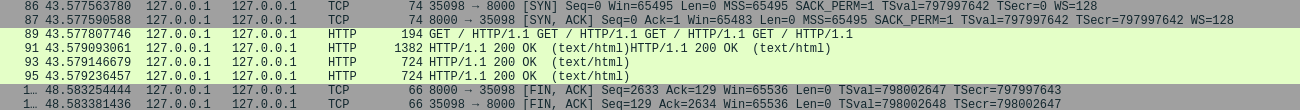
\includegraphics[width=0.95\textwidth]{tests/capture-pipelining.png}
    \caption{Prueba de \key{pipelining}.}
    \label{img-cap-pipelining}
\end{figure}

\end{itemize}

\section{Despliegue de Servicios Telemáticos}
\subsection{Escenario Desarrolado y Versiones del Software}
El escenario objetivo está compuesto por dos equipos distintos conectados a través de una red local. Para simularlo, se ha utilizado el gestor de máquinas virtuales \key{Virtual Box 6.1}.

En un equipo residen los servidores principales de los servicios. Se trata de una instancia de \key{Ubuntu 16.04 Server}. En el otro equipo se encuentra instalado \key{Ubuntu 16.04 Desktop} y cumple el papel de cliente en los servicios. Las dos máquinas virtuales disponen de una tarjeta de red virtual que simula que estuviesen conectadas a la misma red.

\subsection{Servidor DNS}
Uno de los servicios a desplegar era un servidor {\DNS} raíz. El resto de los servicios se apoyan en la resolución de nombres que aporta. Por ejemplo, para que funcione el servidor mail existen dos registros: \code{pop.sstt7628.org} y \code{smtp.sstt7628.org}.

Se eligió la implementación \key{BIND9}, que es el servidor {\DNS} más comúnmente usado en internet y el estándar de facto en sistema UNIX.

\subsubsection{Configuración}
La instalación se llevó a cabo con el gestor de paquetes de \key{Ubuntu}. La configuración depende de varios archivos de texto plano.

En el fichero \file{/etc/bind/named.conf.options} se definen las opciones globales. Se ha configurado que se acepten peticiones de hosts en la red local y que se redirijan las peticiones que no se sepan resolver al servidor {\DNS} de la Universidad de Murcia.

\begin{lstlisting}[title=Fichero \file{/etc/bind/named.conf.options}]
// Para leer todo acerca a la configuración:
// https://www.zytrax.com/books/dns/ch7/
options {
    directory "/var/cache/bind";

    allow-query {        // Hosts que tienen permitido realizar consultas
    	192.168.56.0/24; // Red local de la práctica
    };

    forwarders {    // Direcciones IP de servidores dns para consultas desconocidas.
    	155.54.1.1; // Dirección IP de los servidores DNS de la universidad.
    	155.54.1.2; // Obtenida con el comando dig -t ns um.es
    };

    recursion yes;  // Habilita la recursión para resolver consultas anidadas.
                    // Por ejemplo: www.sstt7628.org (org, sstt7628.org, www.sstt7628.org)

    dnssec-validation auto;

    auth-nxdomain no;     # conform to RFC1035
    listen-on-v6 { any; };
};
\end{lstlisting}

El fichero \file{/etc/bind/named.conf.local} sirve para configurar las zonas que conoce el servidor. Basta con poner que se trata de una zona manejada por nuestro servidor (\key{type master}) y definir un fichero de zona que debemos localizar en la carpeta \file{/etc/bind}. Es habitual, si hay pocos ficheros de zona, que el nombre de los ficheros de zona debe comenzar por \key{db} y no se incluyan dentro de ninguna subcarpeta, pero no es obligatorio.

\begin{lstlisting}[title=Fichero \file{/etc/bind/named.conf.local}]
zone "sstt7628.org." IN {
    type master; // El servidor lee la información de un fichero de zona local
                 // y responde de forma autoritativa.
    file "/etc/bind/db.sstt7628.org.zone"; // El fichero de zona
}
\end{lstlisting}

En el fichero de zona (\key{/etc/bind/db.sstt7628.org.zone}) se configuraron los valores asociados a nuestro dominio, como el \key{TTL} (\textit{time to live}). En mi caso he definido varios registros, entre ellos dos registros de correo electrónico, que se utilizan en el resto de apartados.
\begin{lstlisting}[title=Fichero \file{/etc/bind/db.sstt7628.org.zone}]
; Toda la información de configuración de los ficheros de zona en
; https://www.zytrax.com/books/dns/ch8/
$ORIGIN    sstt7628.org. ; Especificamos que a los nombres que acaben sin un punto
                         ; se les añada esta ruta
$TTL    3600
@         IN    SOA     sstt7628.org. root.sstt7628.org. (
                             1        ; Serial
                          3600        ; Refresh
                          1800        ; Retry
                        604800        ; Expire
                          3600)       ; Negative Cache TTL
;
@         IN    NS      localhost.
cliente   IN    A       192.168.56.101
servidor  IN    A       192.168.56.104
www       IN    CNAME   servidor
web       IN    CNAME   servidor
mail      IN    A       192.168.56.104
@         IN    MX 10   mail
smtp      IN    CNAME   mail
pop       IN    CNAME   mail
\end{lstlisting}

Por otro lado, además de registrar el servidor {\DNS} hay que configurar los hosts para que hagan peticiones a este servidor.

La configuración de dominios {\DNS} se encuentra en el fichero \file{/etc/resolv.conf}. No obstante, los cambios que hagamos sobre este fichero se perderán al reiniciar el ordenador, porque es un fichero generado automáticamente. En su lugar, podemos editar el fichero \file{/etc/resolvconf/resolv.conf.d/head}, que se copia al principio durante la generación. Para añadir un servidor {\DNS} basta con añadir la línea

\begin{center}\code{nameserver 192.168.56.104}.\end{center}

Podemos evitar reiniciar el sistema para ver los cambios ejecutando la orden \code{resolvconf -u}.

\subsubsection{Capturas Wireshark}
A continuación (\cref{img-cap-dns}) se muestra un trozo de la captura Wireshark adjunta donde se ve una consulta {\DNS}.

\begin{figure}[h]
    \centering
    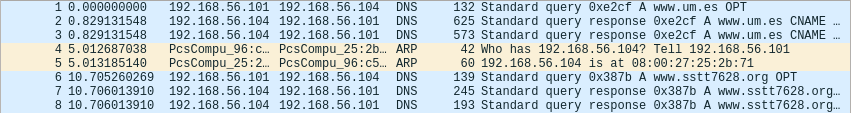
\includegraphics[width=0.95\textwidth]{tests/capture-dns.png}
    \caption{Dos consultas {\DNS}}
    \label{img-cap-dns}
\end{figure}

\subsection{Correo {\SMTP/\POP}}
Se ha desplegado también un servicio de correo electrónico {\SMTP/\POP} mediante las implementaciones \key{exim} y \key{dovecot}. El procedimiento ha sido el explicado en las sesiones de prácticas.

\subsubsection{Usuarios de correo}
Se crearon dos usuarios de correo con nombres \code{nombre1_49277628@sstt7628.org} y \code{nombre2_49277628@sstt7628.org} como pedía la práctica. Con la configuración vista en clase, basta con registrar ambos usuarios en el sistema y el directorio de correo (\key{Mailbox}) se crea automáticamente.

Para verificar el funcionamiento se se utilizó el gestor de correo \key{Thunderbird} (en el cliente) y se enviaron varios correos de una a otra.

\subsubsection{Capturas Wireshark}
A continuación (\cref{img-cap-mail}) se muestra un trozo de la captura Wireshark adjunta donde se muestran los mensajes intercambiados para el envío de un correo electrónico.

\begin{figure}[h]
    \centering
    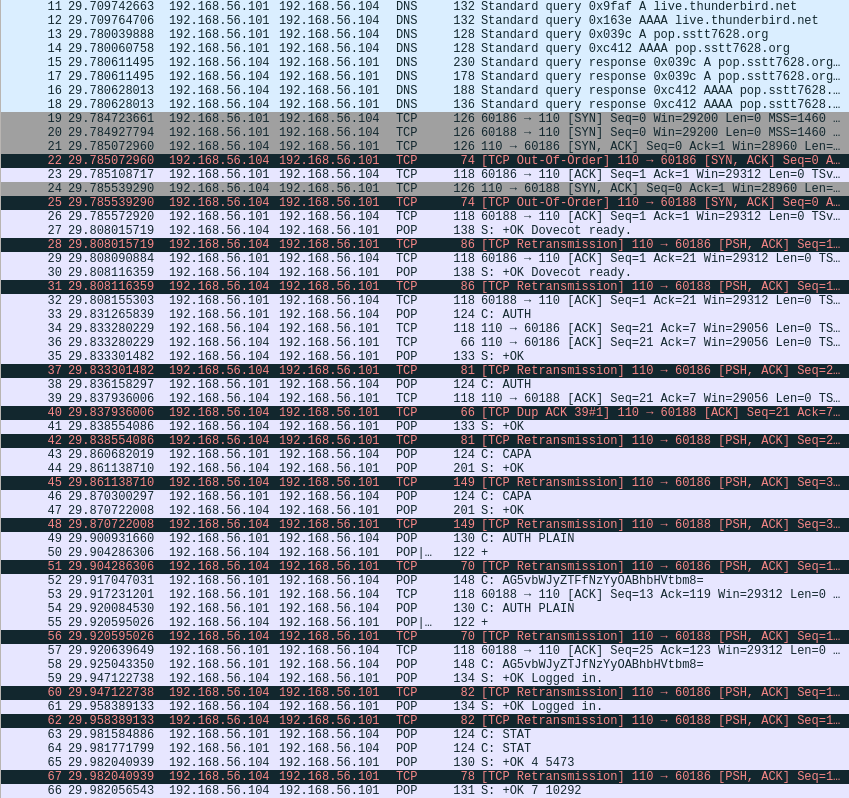
\includegraphics[width=0.95\textwidth]{tests/capture-mail.png}
    \caption{Tráfico generado por Thunderbird}
    \label{img-cap-mail}
\end{figure}

\subsection{Servidor {\HTTP} y {\HTTPs} basado en \key{Apache}}
El grueso del trabajo era implementar el servidor {\HTTP} descrito en la primera sección. No obstante, también hemos tenido que configurar un servidor \key{Apache} que recibiese peticiones {\HTTP} (en el puerto $80$) y {\HTTPs} (en el puerto $443$).

\subsubsection{Configuración}
La configuración se lleva a cabo, una vez más, a través de ficheros de configuración del sistema. Para usar \key{Apache} hay que configurar \key{Virtual Hosts} a través de los siguientes pasos.

\begin{enumerate}
\item Se crea el fichero del sitio \file{/etc/apache2/sites-available/sitio.conf} (Apache incluye ficheros de ejemplo que se pueden utilizar como base). Para la práctica se ha configurado ambos \key{Virtual Hosts} en el mismo fichero porque corresponden al mismo sitio.
\item Se activa el fichero con el comando \code{a2ensite}, que entre otras cosas crea un enlace dinámico a nuestro fichero en la carpeta \file{/etc/apache2/sites-available/}.
\item Y se recarga el servicio de apache (\code{service apache2 reload}), tras lo cual ya podemos acceder.
\end{enumerate}

Si no disponemos de un servicio de {\DNS} que resuelva los nombres de nuestros sitios, podemos añadir una entrada al fichero \file{/etc/hosts}, que sirve para registrar traducciones estáticas en \key{Linux}. En mi caso, instalé \key{Apache} antes de configurar \key{BIND} y ese fue el procedimiento inicial.

El servidor {\HTTP} se protegió mediante usuario y contraseña siguiendo los siguientes pasos.

\begin{itemize}
\item Configuramos el virtual host {\HTTP} de \key{Apache} para restringir la entrada a un grupo de usuarios registrados en ficheros de configuración de \key{Apache}. Es decir, para utilizar un login y contraseña.

\begin{lstlisting}[title=Primera parte del fichero \file{/etc/apache2/sites-available/sstt7628.conf}]
<VirtualHost *:80>
	ServerName www.sstt7628.org

	ServerAdmin admin@sstt7628.org
	DocumentRoot /var/www/sstt7628

	<Directory /var/www/sstt7628>
		AllowOverride AuthConfig
		AuthType Basic
		AuthName "Restricted access to group sstt7628"
		AuthBasicProvider file
		AuthUserFile /etc/apache2/passwords
		AuthGroupFile /etc/apache2/groups
		Require Group sstt7628
			Order allow,deny
			allow from all
	</Directory>

	ErrorLog ${APACHE_LOG_DIR}/error.log
	CustomLog ${APACHE_LOG_DIR}/access.log combined
</VirtualHost>
\end{lstlisting}

\item Los usuarios se crean con el comando \code{htpasswd -c /etc/apache2/passwords sstt7628} y se registran en el grupo añadiendo un fichero \file{groups} en la carpeta donde se encuentre el fichero de usuarios con el siguiente formato
\begin{lstlisting}[title=Fichero \file{/etc/apache2/groups}]
    sstt7628: sstt7628
\end{lstlisting}

\item La configuración de usuarios requiere del módulo \code{authz_groupfile} de \key{Apache}. No hace falta instalarlo en \key{Ubuntu}. Basta con ejecutar el comando \code{a2enmod authz_groupfile} para habilitarlo.
\end{itemize}


\subsection{Certificación {\HTTPs} a través de \key{OpenSSL}}
La configuración del servidor {\HTTPs} es más complicada y requiere que una entidad certificadora firme (en el sentido utilizado en informática para claves públicas y privadas) los certificados que utiliza el protocolo.

Aunque no se ha desplegado una entidad certificadora en el servidor (lo que tendría sentido sería que estuviese en un tercer ordenador), se ha simulado el proceso ejecutando los comandos de la herramienta \key{OpenSSL} tal cual vimos en las clases de prácticas y se encuentra documentado en las diapostivas.

% He utilizado el directorio `~/CAentity`.
% Para generar el primer certificado de la CA he utilizado password como palabra de paso y ca.sstt7628.org como common name.

Una vez generadas las claves para ambos dispositivos y configurado el navegador web del cliente, \key{Firefox} para que reconociese a la entidad certificadora, se configuró el servidor {\HTTPs} en el fichero \file{/etc/apache2/sites-available/sstt7628.conf}.

\begin{lstlisting}[title=Segunda parte del fichero \file{/etc/apache2/sites-available/sstt7628.conf}]
<VirtualHost *:443>
	ServerName www.sstt7628.org

	ServerAdmin admin@sstt7628.org
	DocumentRoot /var/www/sstt7628

	# Authentication Configuration
	SSLEngine on
	# Los ficheros de claves han sido generados usando OpenSSL.
	SSLCertificateFile		/home/alumno/CAentity/servercert.pem
	SSLCertificateKeyFile	/home/alumno/CAentity/serverkey.pem
	SSLCACertificateFile	/home/alumno/CAentity/cacert.pem

	SSLVerifyClient			require
	SSLVerifyDepth			10
</VirtualHost>
\end{lstlisting}

\subsubsection{Capturas Wireshark}
A continuación (\cref{img-cap-http,img-cap-https}) se muestra un trozo de la captura Wireshark adjunta donde se muestra primero un acceso al servidor web vía {\HTTP} y después vía {\HTTPs}.

\begin{figure}[h]
    \centering
    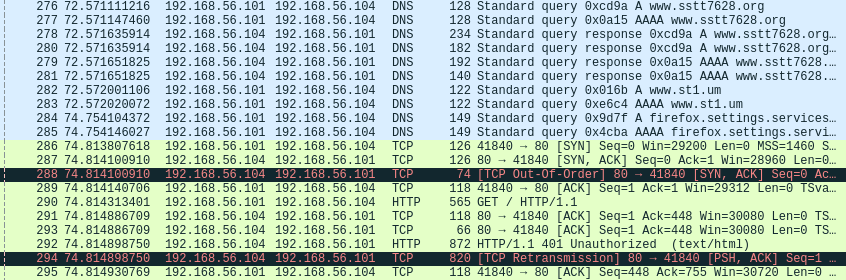
\includegraphics[width=0.95\textwidth]{tests/capture-http.png}
    \caption{Tráfico generado por \key{Firefox} con la petición {\HTTP}}
    \label{img-cap-http}
\end{figure}

\begin{figure}[h]
    \centering
    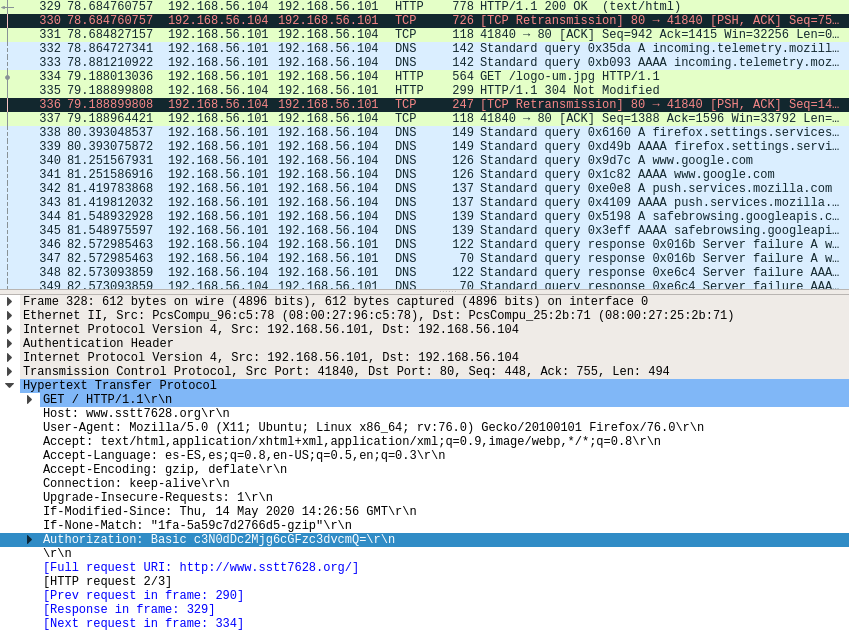
\includegraphics[width=0.95\textwidth]{tests/capture-https.png}
    \caption{Tráfico generado por \key{Firefox} con la petición {\HTTPs}}
    \label{img-cap-https}
\end{figure}


\subsection{IPsec con \key{Strongswan}}
Por último, se pedía implementar el protocolo {\IPsec} para proteger los paquetes {\IP} entre ambos dispositivos. Los requisitos eran utilizar \key{IKEv2} para el establecimiento del canal y operar en modo túnel con autentificación a través de la cabecera \key{AH}, pero sin encriptación. Para ello, se podían utilizar los certificados de identidad que utilizamos para la conexión {\HTTPs}.

Se ha hecho uso de \key{Strongswan}, una implementación \textit{Open Source} de {\IPsec}. Como en el resto de casos, la instalación se ha llevado a cabo a través del gestor de paquetes de \key{Ubuntu}, \code{apt}.

\subsubsection{Configuración}
La configuración de los canales se puede escribir en el fichero \file{/etc/ipsec.conf} de cada host.

\begin{lstlisting}[title=Fichero \file{/etc/ipsec.conf} del servidor]
config setup

conn %deault # Valores por defecto para las conexiones
	ikelifetime=60m
	keylife=20m
	rekeymargin=3m
	keyingtries=1
	mobike=no
	keyexchange=ikev2
	authby=pubkey

conn host-host # Conexión host-host de la práctica
	left=192.168.56.104 # IP del servidor
	leftcert=/etc/ipsec.d/certs/servercert.pem # Clave pública generada con OpenSSL
	leftid="C=ES, ST=Murcia, O=UMU, OU=sstt7628, CN=www.sstt7628.org"
	right=192.168.56.101 # IP del cliente
	rightid="C=ES, ST=Murcia, O=UMU, OU=sstt7628, CN=emilio49277628"
	type=tunnel
	ah=sha256
	auto=start
\end{lstlisting}

\begin{lstlisting}[title=Fichero \file{/etc/ipsec.conf} del cliente]
config setup

conn %deault # Valores por defecto para las conexiones
	ikelifetime=60m
	keylife=20m
	rekeymargin=3m
	keyingtries=1
	mobike=no
	keyexchange=ikev2
	authby=pubkey

conn host-host # Conexión host-host de la práctica
	left=192.168.56.101 # IP del cliente
	leftcert=/etc/ipsec.d/certs/servercert.pem # Clave pública generada con OpenSSL
	leftid="C=ES, ST=Murcia, O=UMU, OU=sstt7628, CN=emilio49277628"
	right=192.168.56.104 # IP del servidor
	rightid="C=ES, ST=Murcia, O=UMU, OU=sstt7628, CN=www.sstt7628.org"
	type=tunnel
	ah=sha256
	auto=start
\end{lstlisting}

En la configuración se puede ver que se ha seleccionado el modo túnel y que se utiliza el protocolo sin encriptación. Concretamente, la línea \code{ah=sha256} especifica que no se utilice encriptación \key{ESP}, el modo predeterminado en \key{Strongswan}. \key{sha256} es una función de hash que se utiliza para asegurar la integridad de los paquetes en la cabecera \key{AH}. Hay muchas opciones disponibles, y he elegido esta función por ser bastante común.

Por último, hay que modificar otro fichero, \file{/etc/ipsec.secrets}, que contiene la información delicada. Lo que hay que incluir en él es la ruta al fichero que contiene la clave privada.

\begin{lstlisting}[title=Fichero \file{/etc/ipsec.secrets} del cliente]
: RSA /etc/ipsec.d/private/clientkey.pem
\end{lstlisting}

\subsubsection{Capturas Wireshark}
A continuación (\cref{img-cap-ping}) se muestra un trozo de la captura Wireshark adjuntada donde se ve que los mensajes originados por un ping de una máquina a otra incluyen la cabecera \key{AH} de {\IPsec}.

\begin{figure}[h]
    \centering
    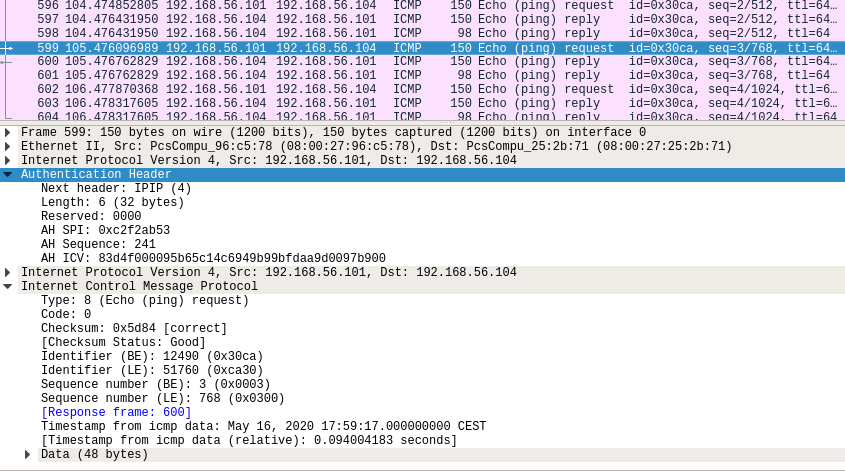
\includegraphics[width=0.95\textwidth]{tests/capture-ping.png}
    \caption{Tráfico generado por el comando \code{ping}. Se ve la cabecera \key{AH}.}
    \label{img-cap-ping}
\end{figure}



\section{Horas de Trabajo}
Para contabilizar las horas trabajadas en esta entrega hemos utilizado la herramienta \key{progesa-test} de la Facultad de Informática. A continuación se puede ver una tabla con el tiempo dedicado a cada apartado de la práctica.

\begin{center}
\begin{tabular}{|p{5cm}|c|}
    \hline
    \multicolumn{2}{|c|}{Entrega Anticipada} \\
    \hline\hline
    \multicolumn{1}{|c|}{Actividad} & Trabajo Autónomo \\
    \hline
    Implementación básica servidor {\HTTP} & \SI{17}{\hour} \SI{24}{\minute} \\
    \hline
    Documentación del servidor {\HTTP} & \phantom{9}\SI{7}{\hour} \SI{39}{\minute} \\
    \hline
    Revisión antes de la primera entrega & \phantom{\SI{99}{\hour}} \SI{35}{\minute} \\
    \hline

    Configuración de los servicios telemáticos & \phantom{0}\SI{7}{\hour} \SI{30}{\minute} \\
    \hline
    % Capturas de tráfico y pruebas & \phantom{0}\SI{2}{\hour} \phantom{\SI{00}{\minute}} \\
    % \hline
    Documentación de los servicios telemáticos & \phantom{0}\SI{2}{\hour} \SI{53}{\minute} \\
    \hline
    Revisión final & \phantom{\SI{00}{\minute}} \SI{40}{\minute} \\
    \hline
    \textbf{TOTAL} & \SI{36}{\hour} \SI{41}{\minute} \\ \hline
\end{tabular}
\end{center}


% \section{Conclusiones}
    % \lstinputlisting[caption=message\_processing.cpp]{../src/message_processing.cpp}
\end{document}
